\section{MVP Wireframe}

Shown below is the MVP Wireframe implemented using Figma.

The full diagram can be found in this \href{https://www.figma.com/file/Sfcv02sNfcQDcNzJZBcMjC/SE?type=design&node-id=1302-148192&mode=design}{Figma link}.

\subsection{Dashboard (Student View)}

\begin{figure}[H]
  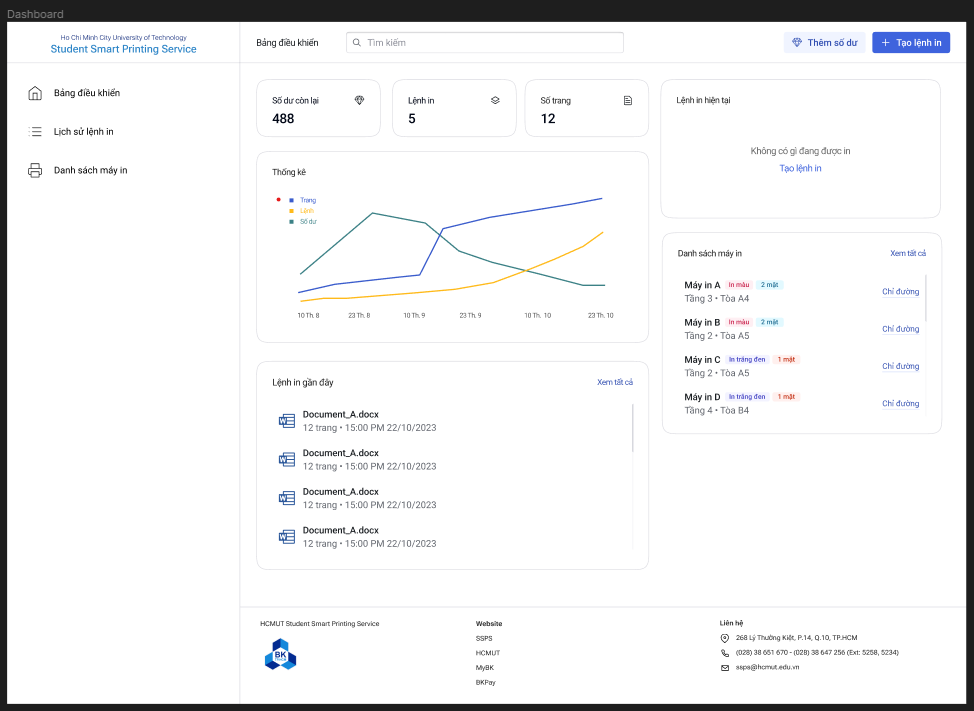
\includegraphics[max width=0.9\linewidth]{chapters/5. mvp-wireframe/1 - Dashboard.png}
  \caption{Dashboard View}%
\end{figure}

The dashboard view allows the user to have quick glance over some basic informations like the amount of balance they have left as well as some printing statistics.\

The sidebar includes links that allow the user to navigate to other features of the application.

\subsection{Create Print Job (Student View)}

From the dashboard, clicking on "Tạo lệnh in" on the top right will open the New Print dialog.

\begin{figure}[H]
  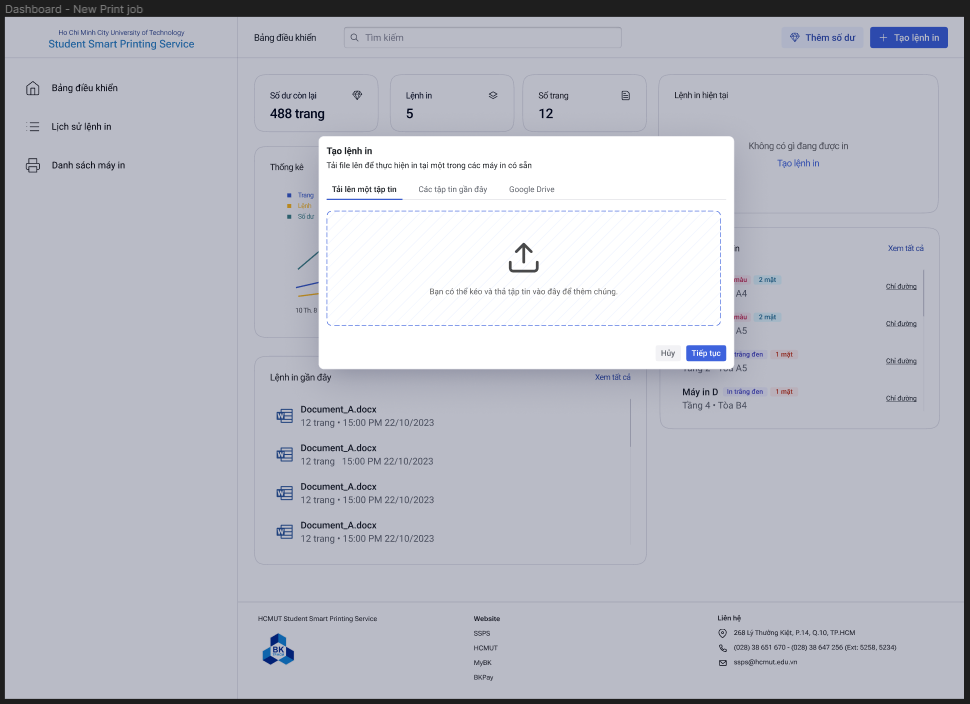
\includegraphics[max width=0.9\linewidth]{chapters/5. mvp-wireframe/2 - Dashboard - Create Print.png}
  \caption{New Print Dialog - Select File}%
\end{figure}

The user can either upload a new file, select a file from those recently uploaded, or select a file from one of the file storage provider integration (Google Drive, OneDrive, etc.).


\begin{figure}[H]
  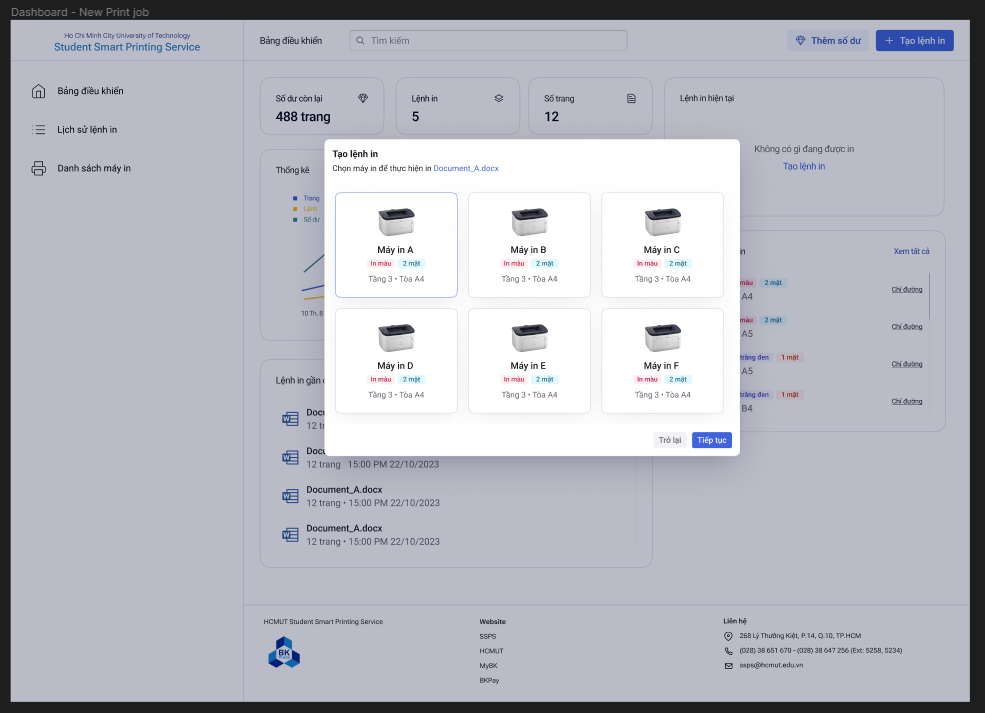
\includegraphics[max width=0.9\linewidth]{chapters/5. mvp-wireframe/3 - Dashboard - Select Printer.png}
  \caption{New Print Dialog - Select Printer}%
\end{figure}

After selecting a file, the user will need to select the printers they would like to use. Each printer card provides the user with information like the printer capabilities as well as its location.

\begin{figure}[H]
  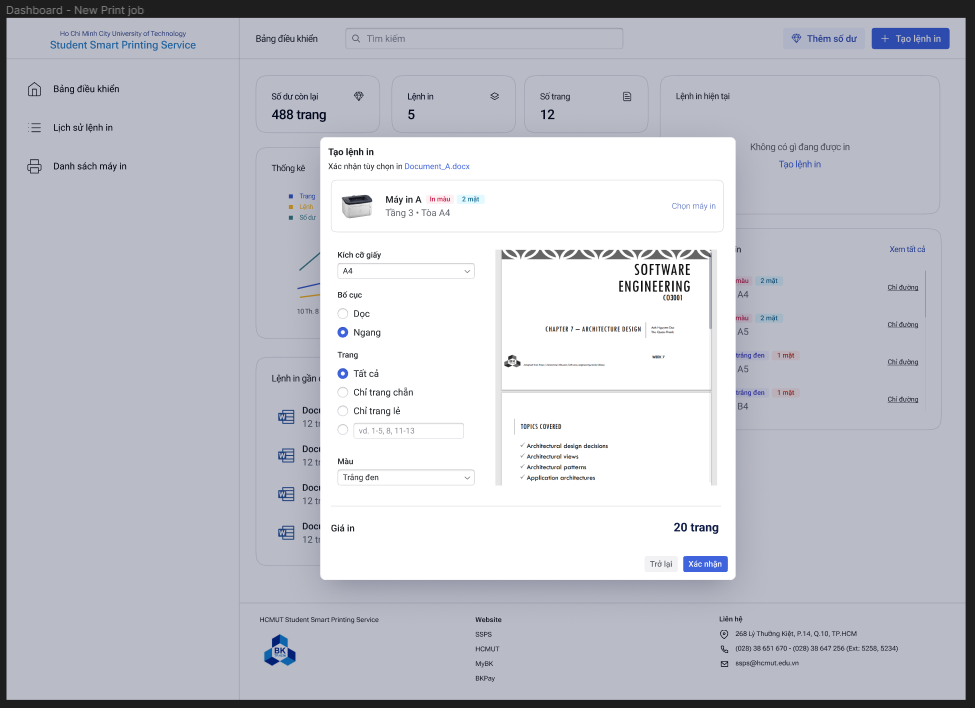
\includegraphics[max width=0.9\linewidth]{chapters/5. mvp-wireframe/4 - Dashboard - Select Properties.png}
  \caption{New Print Dialog - Select Properties}%
\end{figure}

Finally, the user will have to select the properties that they want their file to be printed. The available options will be affected by the configuration of the selected printers.

\subsection{Print History}

\begin{figure}[H]
  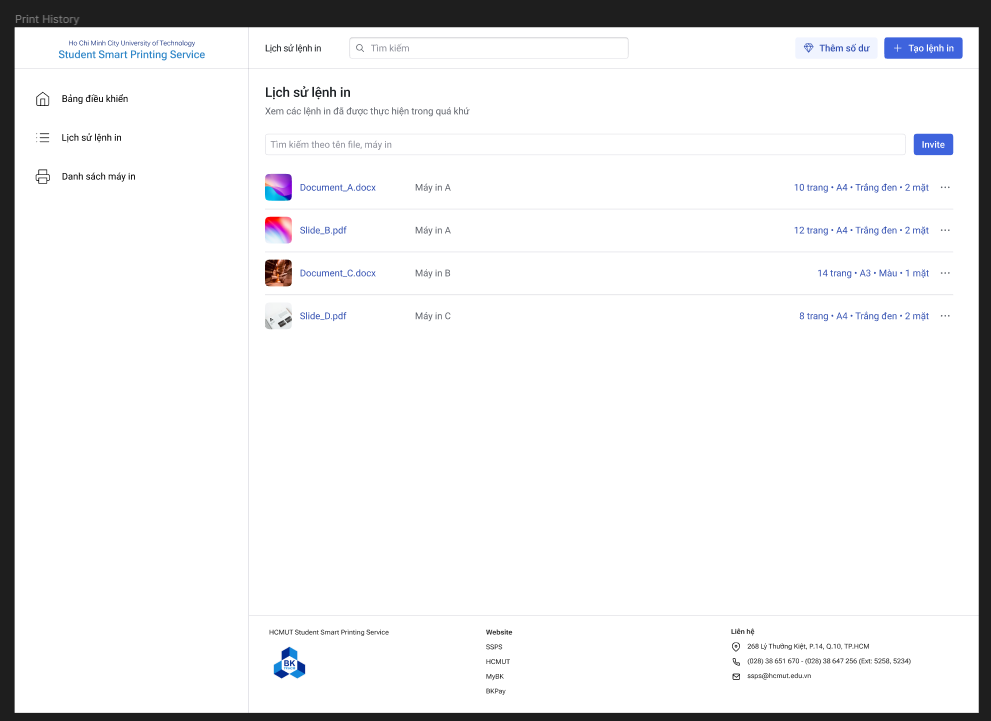
\includegraphics[max width=0.9\linewidth]{chapters/5. mvp-wireframe/5. Print History.png}
  \caption{Print History}%
\end{figure}

The Print History screen allows the user to view all their past print requests as well as the status of ongoing ones.

\begin{figure}[H]
  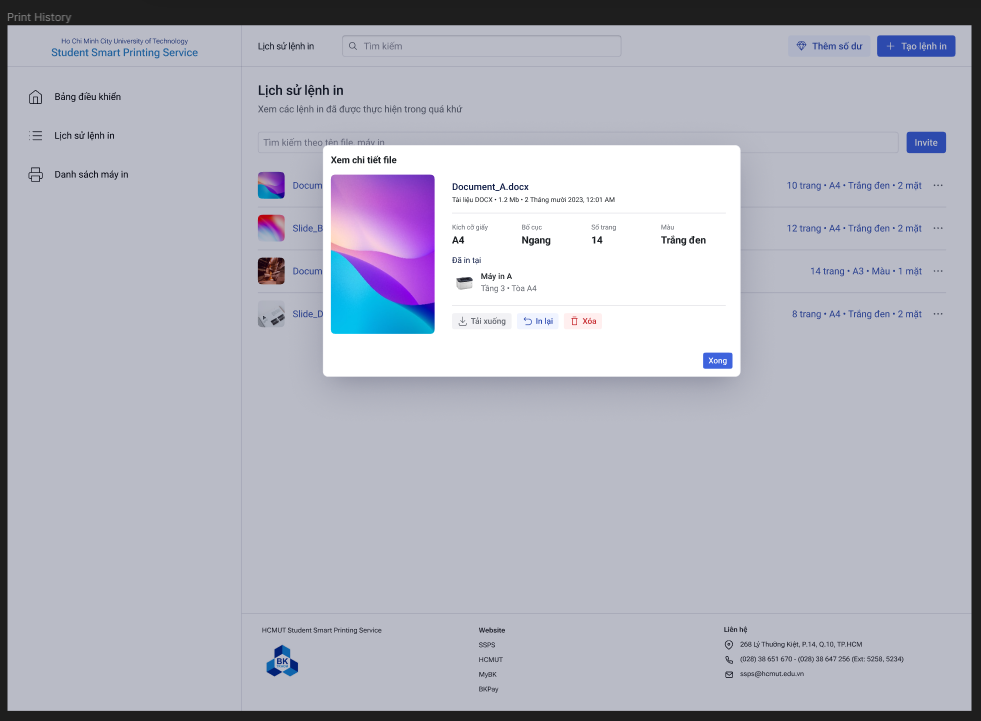
\includegraphics[max width=0.9\linewidth]{chapters/5. mvp-wireframe/6. Print History - Details.png}
  \caption{Print History - Detail view}%
\end{figure}

Clicking on one of the items from the list will open up the detail view, where the user can see all the details as well as performing actions like "Reprint the file", "Download the file", or "Delete the file".

\subsection{Printer List}

\begin{figure}[H]
  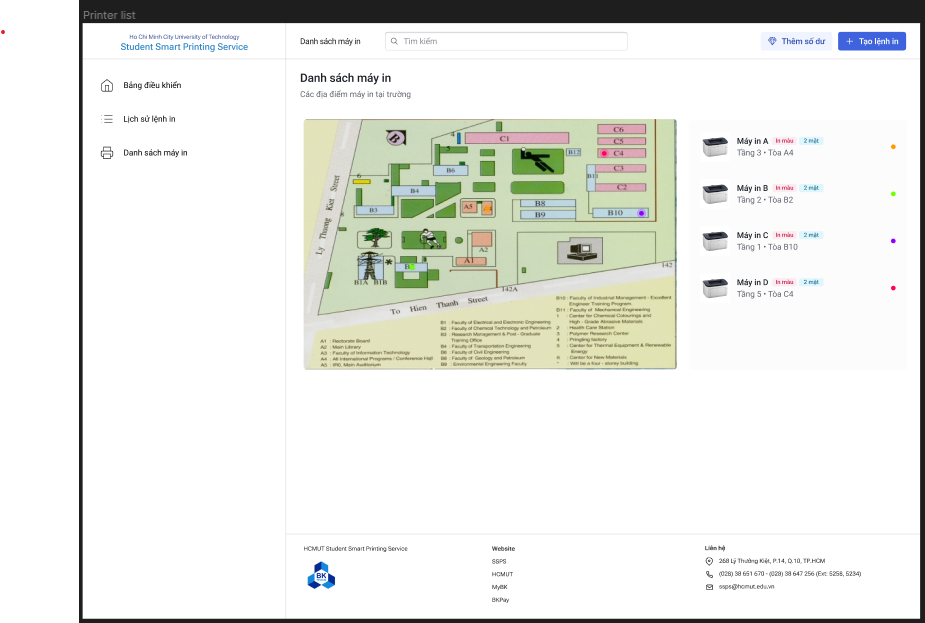
\includegraphics[max width=0.9\linewidth]{chapters/5. mvp-wireframe/7. Printer List.png}
  \caption{Printer List}%
\end{figure}

The Printer List view allows the user to view the list of all printers, their capabilities, and locations.

\begin{figure}[H]
  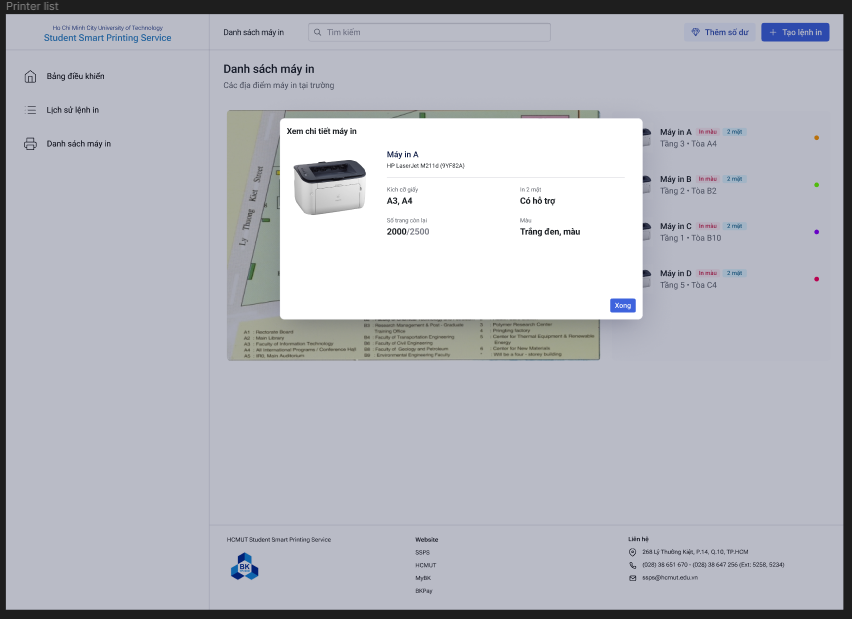
\includegraphics[max width=0.9\linewidth]{chapters/5. mvp-wireframe/8. Printer List - Details.png}
  \caption{Printer List - Detail view}%
\end{figure}

Clicking on one of the printer card will open a detailed view where the user can view all information about the printers.

\subsection{Admin Dashboard View}

The Dashboard admin view can be accessed using the same URL as the one in student view. Depending on the account role, different content is displayed.

\begin{figure}[H]
  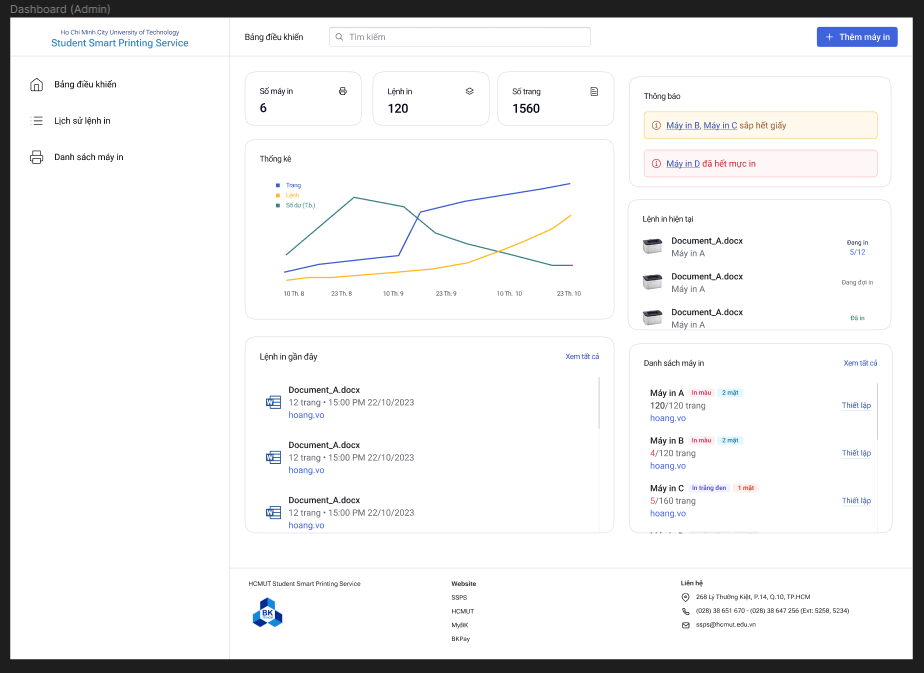
\includegraphics[max width=0.9\linewidth]{chapters/5. mvp-wireframe/9. Dashboard Admin.png}
  \caption{Admin Dashboard}%
\end{figure}

The dashboard admin view also gives the printing statistics but include data from all students.

\subsection{Add Printer}

\begin{figure}[H]
  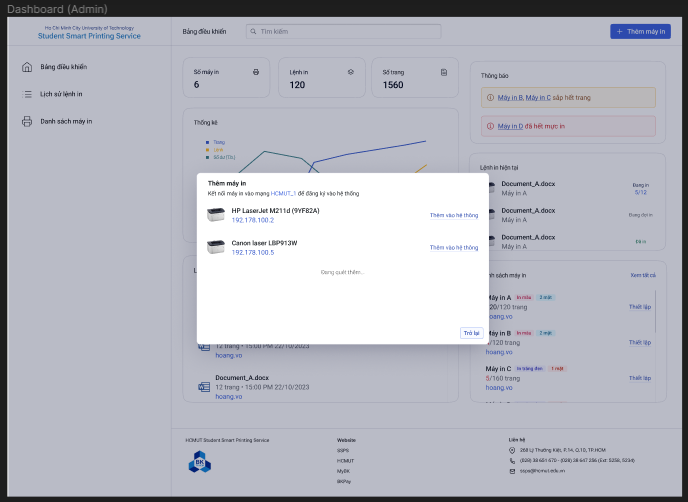
\includegraphics[max width=0.9\linewidth]{chapters/5. mvp-wireframe/10. Add Printer.png}
  \caption{Add Printer}%
\end{figure}

The admin can add new printers using the "Thêm máy in" button in the top right. After that the user can select a printer that can be discovered in the network or enter an IP Address.

\begin{figure}[H]
  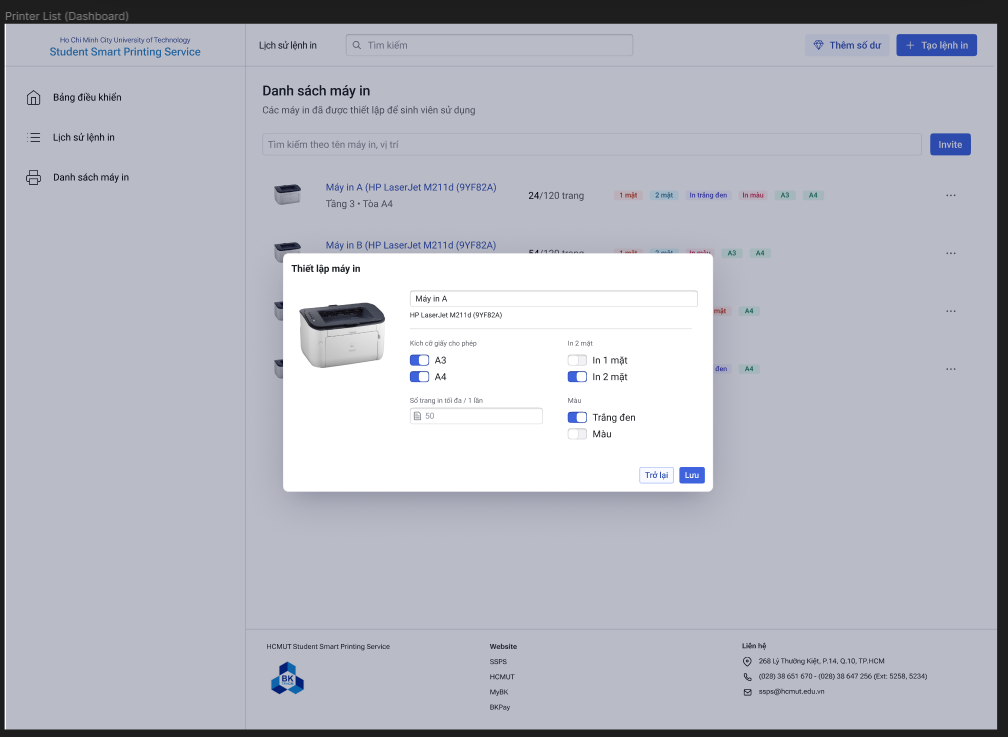
\includegraphics[max width=0.9\linewidth]{chapters/5. mvp-wireframe/12. Admin Printer Edit.png}
  \caption{Configure Printer}%
\end{figure}

The user can then configure the properties of the printers, which will determine the available options when users create a print request.

\subsection{Admin Printer List}

\begin{figure}[H]
  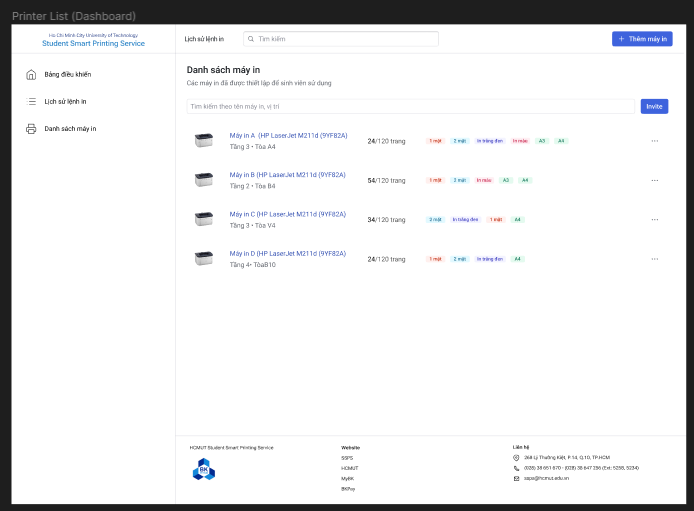
\includegraphics[max width=0.9\linewidth]{chapters/5. mvp-wireframe/11. Admin Printer List.png}
  \caption{Admin Printer List}%
\end{figure}

The admin printer list shows all printers as well as their configuration. Clicking on one of them will open up the printer configuration dialog as seen above.